\documentclass[11pt,letterpaper]{article}
\usepackage{fullpage}
\usepackage{multicol}
\usepackage{amsmath}
\usepackage{amsfonts}
\usepackage{amssymb}
%\usepackage{pstricks, pst-node, pst-plot}

\ifx\pdfoutput\undefined
% we are running LaTeX, not pdflatex
\usepackage{graphicx}
\else
% we are running pdflatex, so convert .eps files to .pdf
\usepackage[pdftex]{graphicx}
\usepackage{epstopdf}
\fi

\newcommand{\ds}{\displaystyle}
\newcommand{\bv}{\mathbf}
\newcommand{\lv}{\langle}
\newcommand{\rv}{\rangle}

\begin{document}
\flushleft
\begin{multicols}{2}


\begin{large}\textbf{Math 116 Quiz 3: $\oint$ 7.5, 8.1-8.2 (sans arc length) \\
Tue 25 Sep 2012}\end{large}

\textbf{Name:  }\underline{\hspace{4pc}{\bf SOLUTIONS}\hspace{4pc}}
\vspace{.5in}

\end{multicols}

\pagestyle{empty}

\flushleft

You have 30 minutes to complete this quiz.  Eyes on your own paper and good luck!

\begin{enumerate}

\item \textbf{Definitions/Concepts.} (2 pts) Fill in the following inequalities using the symbols TRAP$(n)$ or MID$(n)$.  

\smallskip
If the graph of $f$ is concave down on $[a,b]$, then
\[\text{TRAP$(n)$   }\leq\int_a^bf(x)dx\leq\text{   MID$(n)$}\]
If the graph of $f$ is concave up on $[a,b]$, then
\[\text{MID$(n)$   }\leq\int_a^bf(x)dx\leq\text{   TRAP$(n)$}\]

\vspace{1pc}
\item \textbf{Questions/Problems.} (8 pts)
\noindent Let $S$ be the solid whose base is the region bounded by the graph of the curve $y=\frac{1}{\sqrt{x(1+a\ln\,x)}}$ (for some positive constant $a>0$), the $x$-axis, the lines $x=1$ and $x=e$.  The cross-sections of $S$ perpendicular to the $x$-axis are squares.  Find the exact volume of $S$.
\smallskip
\begin{center}
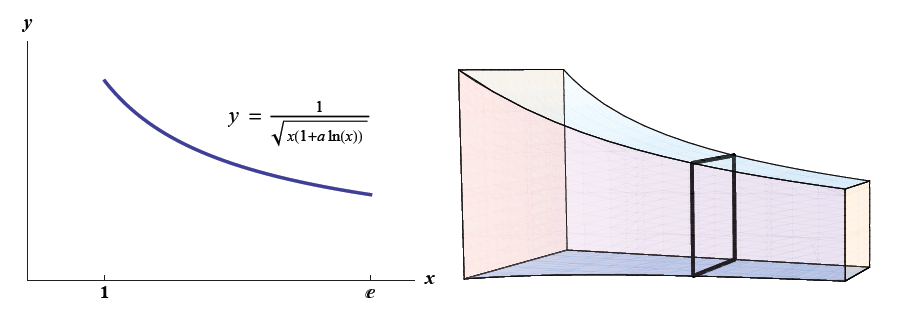
\includegraphics[width=.9\textwidth]{quiz3pic.png}
\end{center}

The volume of one infinitessimal slice will be the area of the square multiplied by a width $dx$.  The length of one side of the square is given by $\frac{1}{\sqrt{x(1+a\ln\,x)}}$.  Now we can compute the total volume using an integral
\[V=\int_1^e\frac{dx}{x(1+a\ln{x})}.\]
The most efficient way to evaluate this integral is to use the substitution $w=1+a\ln{x}$, $dw=\frac{a}{x}dx$.  Now we evaluate the indefinite integral:
\[\frac{1}{a}\int\frac{dw}{w}=\frac{1}{a}\ln{|w|}\]
Resubstituting to get an expression in terms of $x$ and applying the bounds of integration gives
\[\left.\frac{1}{a}\ln{|1+a\ln{x}|}\right|_1^e=\frac{1}{a}\ln{|1+a|}.\]
In fact, since we are told $a>0$ we can drop the absolute value signs to get $\frac{1}{a}\ln{(1+a)}$.

%\vfill
%\hfill{\bf MORE QUIZ ON THE BACK --\textgreater}
\vspace{1pc}
\item \textbf{Computations/Algebra.} 

\smallskip
\begin{enumerate} 
\item $\int_0^6\pi(3-y/2)^2dy$
\smallskip
\begin{enumerate}
\item (1 pt) Which shape is being integrated?  Choose one:
\begin{enumerate}
\item triangle
\item part of a circle
\item hemisphere
{\bf\item cone}
\end{enumerate}
\smallskip
\item (2 pts) If you chose triangle, write down the base and height, indicating which is which.  If you chose part of a circle or hemisphere, write down the radius.  If you chose cone, write down the radius and the height, indicating which is which.

\vspace{0.5pc}
radius = $3-\frac{y}{2}$ \\
height = $6$

\vspace{0.5pc}
\item (2 pts) Draw a picture to justify your answers to parts i. and ii.
\smallskip
\begin{center}
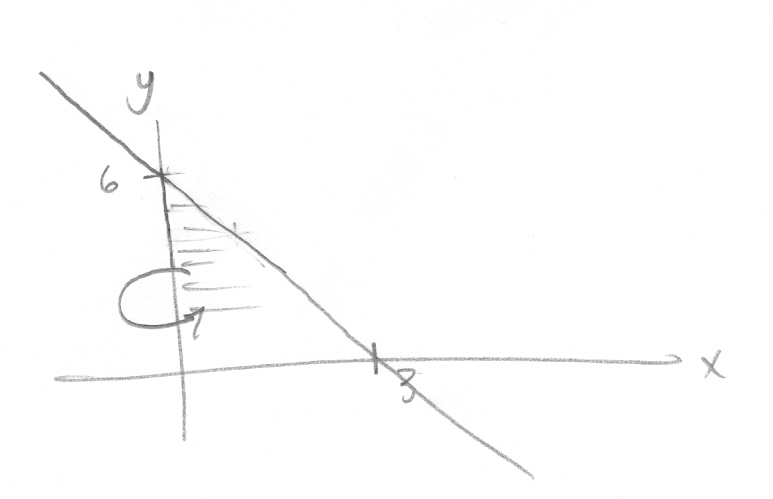
\includegraphics[width=.2\textwidth]{scan0011.jpg}
\end{center}
\vspace{1pc}
\end{enumerate}

\item $\int_{-9}^9\sqrt{81-x^2}dx$
\smallskip
\begin{enumerate}
\item (1 pt) Which shape is being integrated?  Choose one:
\begin{enumerate}
\item triangle
{\bf\item part of a circle}
\item hemisphere
\item cone
\end{enumerate}
\smallskip
\item (2 pts) If you chose triangle, write down the base and height, indicating which is which.  If you chose part of a circle or hemisphere, write down the radius.  If you chose cone, write down the radius and the height, indicating which is which.

\vspace{0.5pc}
radius = $9$ 

\vspace{4pc}
\item (2 pts) Draw a picture to justify your answers to parts i. and ii.
\smallskip
\begin{center}
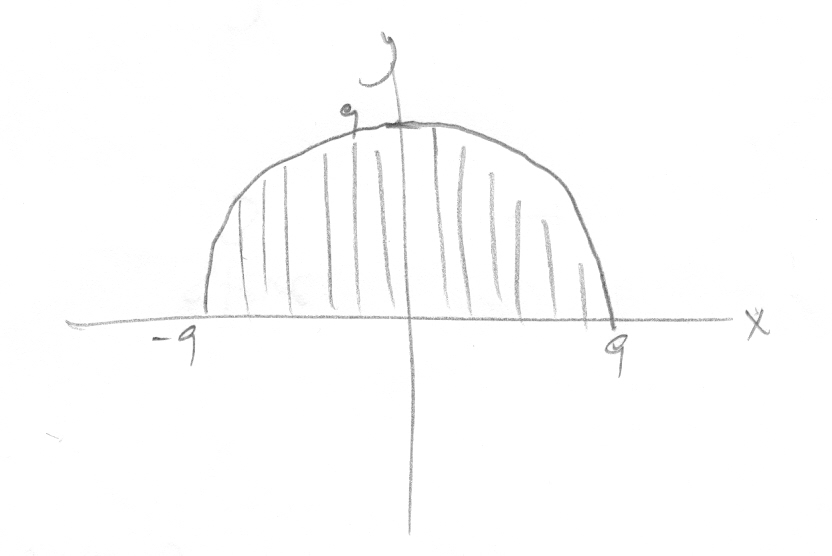
\includegraphics[width=.2\textwidth]{scan0012.jpg}
\end{center}
\vspace{0.5pc}
\end{enumerate}

\end{enumerate}

\end{enumerate}

{\bf ChAlLeNgE pRoBlEm:} Rotate the bell curve $y=e^{-x^2/2}$ around the $y$-axis, forming a hill-shaped solid of revolution.  Using horizontal slices, find the exact volume of this hill.

\vspace{0.5pc}
We will integrate discs of thickness $dy$.  The radius of each disc is half of the length of the horizonal strip.  We can get the radius exactly by solving for the $x$-coordinate:
\begin{align*}
y &=e^{-x^2/2} \\
\ln{y} &= \frac{-x^2}{2} \\
-2\ln{y} &=x^2 \\
\ln{y^{-2}} &= x^2 \\
\ln{\frac{1}{y^2}} &= x^2 \\
\sqrt{\ln{\frac{1}{y^2}}} &= x
\end{align*}

As $x\to\pm\infty$ the bell curve approaches $0$, so we integrate $y$ from $\gamma$ to $1$ ($\gamma$ will be a ``dummy" variable representing $y$) and take the limit as $\gamma$ approaches zero.
\begin{align*}
\pi\int_{\gamma}^1\left(\sqrt{\ln{\frac{1}{y^2}}}\right)^2dy &= \pi\int_{\gamma}^1\ln{\frac{1}{y^2}}\,dy \\
&= \pi\int_{\gamma}^1-2\ln{y}\,dy \\
&= -2\pi\int_{\gamma}^1\ln{y}\,dy \\
\text{(see p. 343 of the text on how to integrate natural log)   } &= -2\pi\left(y\ln{y}|_{\gamma}^1-\int_{\gamma}^1dy\right) \\
&= -2\pi\left(1\cdot\ln{1}-\gamma\cdot\ln{\gamma}-(1-\gamma)\right) \\
&= -2\pi(-\gamma\ln{\gamma}-1+\gamma) 
\end{align*}
At this point the limit
\[\lim_{\gamma\to 0}\gamma\ln{\gamma}\]
is $0\cdot(-\infty)$, which is not well-defined.  However, we can apply L'H\^opital's rule by writing
\begin{align*}
\lim_{\gamma\to 0}\gamma\ln{\gamma} &=\lim_{\gamma\to 0}\frac{\ln{\gamma}}{\frac{1}{\gamma}} \\
&=\lim_{\gamma\to 0}\frac{\frac{d}{d\gamma}\left(\ln{\gamma}\right)}{\frac{d}{d\gamma}\left(\frac{1}{\gamma}\right)} \\
&=\lim_{\gamma\to 0}\frac{\frac{1}{\gamma}}{-\frac{1}{\gamma^2}} \\
&=\lim_{\gamma\to 0}-\gamma \\
&=0.
\end{align*}
Then taking the limit of the integral, we get
\begin{align*}
\lim_{\gamma\to 0}-2\pi(-\gamma\ln{\gamma}-1+\gamma) &= -2\pi(0-1+0) \\
&=2\pi.
\end{align*}

\end{document}


